% 
% funCKit - functional Circuit Kit
% Copyright (C) 2013  Lukas Elsner <open@mindrunner.de>
% Copyright (C) 2013  Peter Dahlberg <catdog2@tuxzone.org>
% Copyright (C) 2013  Julian Stier <mail@julian-stier.de>
% Copyright (C) 2013  Sebastian Vetter <mail@b4sti.eu>
% Copyright (C) 2013  Thomas Poxrucker <poxrucker_t@web.de>
% Copyright (C) 2013  Alexander Treml <alex.treml@directbox.com>
% 
% This program is free software: you can redistribute it and/or modify
% it under the terms of the GNU General Public License as published by
% the Free Software Foundation, either version 3 of the License, or
% (at your option) any later version.
% 
% This program is distributed in the hope that it will be useful,
% but WITHOUT ANY WARRANTY; without even the implied warranty of
% MERCHANTABILITY or FITNESS FOR A PARTICULAR PURPOSE.  See the
% GNU General Public License for more details.
% 
% You should have received a copy of the GNU General Public License
% along with this program.  If not, see <http://www.gnu.org/licenses/>.
% 


%KOMA-Script (duerfte besser sein für europäische Formate):
%http://www.komascript.de/
\documentclass[12pt,a4paper]{scrartcl}


% configuration
\newcommand{\myStdColor}{\color{black}}
\newcommand{\projectName}{funCKit\xspace} % short name
\newcommand{\fullProjectName}{functional Circuit Kit\xspace} % long name
\newcommand{\headerPageColor}{lightgray}
\newcommand{\headerTextColor}{black}
\newcommand{\headerHighlightTextColor}{HKS41-100}
\newcommand{\funCKit}{
\includegraphics[height=11pt]{../images/funCKit}}

% names of FunCKit
\newcommand{\fckNewBrickList}{Neue-Baustein-Liste\xspace}
\newcommand{\fckMenuBar}{Men\"{u}leiste\xspace}
\newcommand{\fckProjectTree}{Projektbaum\xspace}
\newcommand{\fckToolBar}{Werkzeugset\xspace}
\newcommand{\fckToolBars}{Werkzeugsets\xspace}
\newcommand{\fckNewBrickTool}{Neuer-Baustein - Werkzeug\xspace}
\newcommand{\fckWireTool}{Kabel - Werkzeug\xspace}
\newcommand{\fckSelectTool}{Auswahl - Werkzeug\xspace}
\newcommand{\fckMoveViewportTool}{Ansicht-verschieben - Werkzeug\xspace}
\newcommand{\fckLiveValidation}{Echtzeitvalidierung\xspace}
\newcommand{\fckEditPanel}{Editierfenster\xspace}
\newcommand{\fckTab}{Reiter\xspace}
\newcommand{\fckTabs}{Reiter\xspace}
\newcommand{\fckOpenDialog}{Öffnen Dialog\xspace}
\newcommand{\fckSEPFormat}{SEP-Austauschformat\xspace}
\newcommand{\fckSEPFormatGenitive}{SEP-Austauschformates\xspace}

% using glossaries
\usepackage[toc]{glossaries}
% used for wrapping images
\usepackage{wrapfig}
% Den Punkt am Ende jeder Beschreibung im Glossar deaktivieren
\renewcommand*{\glspostdescription}{}
\makeglossary

% header file
\input{../header}

% Make sections blue .. looks cooler ;)
\addtokomafont{section}{\color{HKS41-100}}

%% only import vc.tex if exists
\newboolean{vc_is_included}
\InputIfFileExists{vc.tex}{\setboolean{vc_is_included}{true}}{\setboolean{vc_is_included}{false}}

% ____________________
% |                   |
% |      Header       |
% |                   |
% | > http://de.wikibooks.org/wiki/LaTeX-W%C3%B6rterbuch:_fancyhdr
% |___________________|
%
\pagestyle{fancy} %eigener Seitenstil
\fancyhf{} %alle Kopf- und Fußzeilenfelder bereinigen
\fancyhead[L]{\color{HKS41-100}\projectName} %Kopfzeile links
\fancyhead[C]{\ifthenelse{\boolean{vc_is_included}}{(\VCRevision/\VCAuthor/\VCDateTEX/\VCTime)}{}} %zentrierte Kopfzeile
\fancyhead[R]{\color{HKS41-100}\nouppercase{\leftmark}} %Kopfzeile rechts
\renewcommand{\headrulewidth}{0.4pt} %obere Trennlinie
\fancyfoot[R]{\thepage \space von \pageref{LastPage}} %Seitennummer
%\renewcommand{\footrulewidth}{0.4pt} %untere Trennlinie
\setlength{\skip\footins}{1cm}
% Headerhöhe vergrößern (default: 12pt), andernfalls meckert fancyhdr
\setlength{\headheight}{26pt}
% -----------------------------------------------------------------------------

% ____________________
% |                   |
% |     Document      |
% |___________________|
%
\begin{document}
	% ____________________
	% |                   |
	% |    Titlepage      |
	% |___________________|
	%
	\begin{titlepage}
		\pagecolor{\headerPageColor}
		\color{\headerTextColor}
		~ \\
		~ \\
		{\centering
			
\includegraphics[width=0.5\textwidth]{../images/funCKit_logo1}\\
			~ \\
			~ \\
			~ \\
			\dividingRule{black} \\
			~ \\
			\textbf{\color{\headerHighlightTextColor}\scalefont{2.8} Handbuch} \protect\\
			\dividingRule{black} \\
			~ \\
			~ \\
			~ \\
			{\color{\headerHighlightTextColor}\scalefont{1.2}Software Engineering Praktikum} \protect\\
			{\color{\headerTextColor}Wintersemester \textbf{2011/2012}} \protect\\
			~ \\
			~ \\
			{\color{\headerTextColor}\scalefont{0.9}
				\textbf{Auftraggeber Universität Passau} \\
				Dr. Christian Bachmaier, Innstraße 33, 94032 Passau \\
				Fakultät für Informatik und Mathematik \\
				Betreuer: Andreas Gleißner
			}
			\vspace{\fill}
			
			\ifthenelse{\boolean{vc_is_included}}{
			\color{\headerTextColor}
			\textbf{Git-Revision: \VCRevision} \\
			Last Author: \VCAuthor \\
			Last Commit Message: \\
			\VCCommitMessage \\ % watch out: some commit messages could contain character, that will not compile
			Date: \VCDateTEX \\
			Time: \VCTime \\
			\vspace{1cm} }{}
		}

		{\noindent
			\textbf{Team 3} (\textit{team3@sep2011.de}) \\
			Peter Dahlberg (\textit{dahlberg@fim.uni-passau.de}) \\
			Lukas Elsner (\textit{friends@ccube.de}) \\
			Thomas Poxrucker (\textit{poxrucker\_t@web.de}) \\
			Julian Stier (\textit{mail@julian-stier.de}) \\
			Alexander Treml (\textit{alex.treml@directbox.com}) \\
			Sebastian Vetter (\textit{funckit@b4sti.eu})
		}

		\vspace{1cm}

		\raggedleft{\scalefont{0.7}\noindent
			Passau, den \today \\
			Team 3 - Version 1.0
		}

		\color{black}
	\end{titlepage}

  \pagecolor{white}
  \tableofcontents

% ____________________
% |                   |
% |     Glossary      |
% |___________________|
%
% 
% funCKit - functional Circuit Kit
% Copyright (C) 2013  Lukas Elsner <open@mindrunner.de>
% Copyright (C) 2013  Peter Dahlberg <catdog2@tuxzone.org>
% Copyright (C) 2013  Julian Stier <mail@julian-stier.de>
% Copyright (C) 2013  Sebastian Vetter <mail@b4sti.eu>
% Copyright (C) 2013  Thomas Poxrucker <poxrucker_t@web.de>
% Copyright (C) 2013  Alexander Treml <alex.treml@directbox.com>
% 
% This program is free software: you can redistribute it and/or modify
% it under the terms of the GNU General Public License as published by
% the Free Software Foundation, either version 3 of the License, or
% (at your option) any later version.
% 
% This program is distributed in the hope that it will be useful,
% but WITHOUT ANY WARRANTY; without even the implied warranty of
% MERCHANTABILITY or FITNESS FOR A PARTICULAR PURPOSE.  See the
% GNU General Public License for more details.
% 
% You should have received a copy of the GNU General Public License
% along with this program.  If not, see <http://www.gnu.org/licenses/>.
% 


\newglossaryentry{cmd-esc}{
  name=ESC,
  description={
    Die ESC-Taste  }
  }

\newglossaryentry{cmd-scroll}{
  name=Scrollrad,
  description={
    Das Scrollrad der Maus. Bei Betätigung lässt es sich horizontal scrollen.
  }
}
\newglossaryentry{cmd-strg-scroll}{
  name=Strg+Scroll,
  description={
    Bei gedrückter Taste lässt sich bei Betätigung des Scrollrades zoomen.
   }
}
\newglossaryentry{cmd-alt-scroll}{
  name=Alt+Scroll,
  description={
    Bei gedrückter Taste lässt sich bei Betätigung des Scrollrades vertikal scrollen.
  }
}
\newglossaryentry{cmd-cmd}{
  name=Cmd,
  description={
Die Command-Taste bei Mac OS X. Wechselt in den Zoom-Modus und tritt in Verbindung mit anderen Tasten oft in anderen Kombinationen auf.
  }
}

\newglossaryentry{cmd-strg}{
  name=Strg,
  description={
Die Steuerung-Taste. Wechselt in den Zoom-Modus und tritt in Verbindung mit anderen Tasten oft in anderen Kombinationen auf.
  }
}

\newglossaryentry{cmd-strg-1}{
  name=Strg+1,
  description={
	Wechselt in den Selektions-Modus.
  }
}

\newglossaryentry{shift}{
  name=Shift (gedrückt),
  description={
	Wechselt temporär während die Taste gedrückt ist in den Selektions-Modus.
  }
}

\newglossaryentry{space}{
  name=Leertaste (gedrückt),
  description={
	Wechselt temporär während die Taste gedrückt ist in den Ansicht-verschieben-Modus.
  }
}

\newglossaryentry{newbricklist}{
  name=Neue-Baustein-Liste,
  description={
	Bietet eine Auswahl an Bausteinen die zum Erstellen ausgewählt werden können.
  }
}

\newglossaryentry{cmd-strg-2}{
  name=Strg+2,
  description={
	Wechselt in den Hinzufügen-Modus.
  }
}

\newglossaryentry{cmd-strg-3}{
  name=Strg+3,
  description={
	Wechselt zum Kabelwerkzeug.
  }
}

\newglossaryentry{cmd-strg-4}{
  name=Strg+4,
  description={
	Wechselt in den Ansicht verschieben - Modus.
  }
}
\newglossaryentry{cmd-strg-a}{
  name=Strg+A,
  description={
	Markiert alle Elemente im Gitternetz.
  }
}
\newglossaryentry{cmd-space}{
  name=Leertaste (gedrückt),
  description={
	Wechselt in den Ansicht verschieben - Modus.
  }
}


\newglossaryentry{cmd-strg-t}{
  name=Strg+T,
  description={
	Öffnet einen neuen Tab der aktuell geöffneten Schaltung.
  }
}

\newglossaryentry{cmd-strg-w}{
  name=Strg+W,
  description={
	Schließt den aktuellen Tab.
  }
}

\newglossaryentry{cmd-strg-n}{
  name=Strg+N,
  description={
	Neues Projekt öffnen.
  }
}

\newglossaryentry{cmd-strg-o}{
  name=Strg+O,
  description={
	Gespeichertes Projekt öffnen.
  }
}

\newglossaryentry{cmd-strg-s}{
  name=Strg+S,
  description={
	Projekt speichern.
  }
}

\newglossaryentry{cmd-strg-shift-s}{
  name=Strg+Umschalt+S,
  description={
	Projekt speichern unter.
  }
}

\newglossaryentry{cmd-strg-e}{
  name=Strg+E,
  description={
	Komponente exportieren.
  }
}

\newglossaryentry{cmd-strg-q}{
  name=Strg+Q,
  description={
	Programm beenden.
  }
}

\newglossaryentry{cmd-strg-z}{
  name=Strg+Z,
  description={
	Rückgängigmachen von Editieraktionen.
  }
}

\newglossaryentry{cmd-strg-y}{
  name=Strg+Y,
  description={
	Wiederherstellen von Editieraktionen.
  }
}

\newglossaryentry{cmd-strg-x}{
  name=Strg+X,
  description={
	Ausschneiden eines markiertes Bereichs.
  }
}

\newglossaryentry{cmd-strg-c}{
  name=Strg+C,
  description={
	Kopieren eines markiertes Bereichs.
  }
}

\newglossaryentry{cmd-strg-v}{
  name=Strg+V,
  description={
	Einfügen eines davor kopierten Bereichs.
  }
}


\newglossaryentry{cmd-entf}{
  name=Entf,
  description={
	Löschen eines markierten Bereichs.
  }
}
\newglossaryentry{cmd-f11}{
  name=F11,
  description={
	Anzeigen des Programms in Vollbild.
  }
}

\newglossaryentry{cmd-strg-plus}{
  name=Strg+Plus,
  description={
	Vergrößert die Ansicht des Editierpanels.
  }
}

\newglossaryentry{cmd-strg-minus}{
  name=Strg+Minus,
  description={
	Verkleinert die Ansicht des Editierpanels.
  }
}


\newglossaryentry{cmd-strg-0}{
  name=Strg+0,
  description={
	Zoom auf 100-Prozent.
  }
}

\newglossaryentry{cmd-strg-g}{
  name=Strg+G,
  description={
	Anzeige des Gitternetzes.
  }
}
\newglossaryentry{cmd-f1}{
  name=F1,
  description={
	Anzeige des Benutzerhandbuches.
  }
}

\newglossaryentry{Projekt}{
  name=Projekt,
  plural=Projekte,
  description={
       Ein Projekt besteht aus einer Hauptschaltung und bestimmten Zusatzinformationen wie einem Namen. Ein Projekt kann sowohl in eine Datei gespeichert werden als auch aus einer Datei geladen werden.
  }
}

\newglossaryentry{Komponente}{
  name=Komponente,
  description={
    Eine Komponente ist eine \gls{Schaltung} mit benannten Ein- und Ausgängen, die als Baustein in anderen Schaltungen verwendet werden kann.
  },
  plural=Komponenten
}
\newglossaryentry{Schaltung}{
  name=Schaltung,
  description={
    Eine Schaltung ist eine Menge von Bausteinen oder \glspl{Komponente}, die mit Leitungen verbunden sind.
  },
  plural=Schaltungen
}

\newglossaryentry{Tooltip}{
  name=Tooltip,
  description={
    Kästchen mit Informationen, die beim Überfahren eines Elements mit der Maus innerhalb der Benutzeroberfläche angezeigt werden.
  },
  plural=Tooltips
}


% ____________________
% |                   |
% |     Content       |
% |___________________|
%

\newpage
\section{Einleitung}
		\begin{figure}[H]
			\centering
			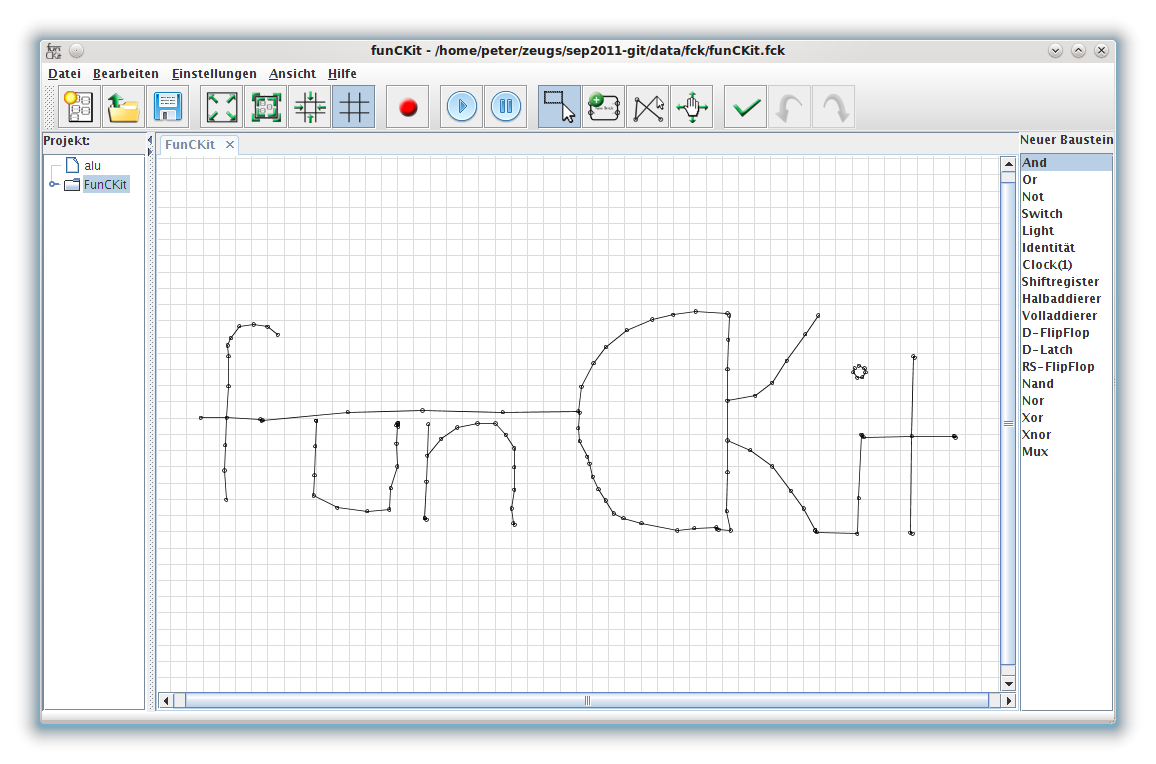
\includegraphics[width=\linewidth]{images/funCKit.png}
			\label{fig:funckit-drawing}
			\caption{funCKit}
		\end{figure}
\funCKit~(\textit{Functional Circuit Kit}; englisch für \textit{Funktionales / fachliches Schaltungswerkzeug}) ist eine Modellierungs- und Simulationssoftware für logische Schaltungen. Sie ermöglicht - aufbauend auf grundlegenden Logikgattern - das Erstellen, Editieren, Simulieren, Austauschen und Untersuchen von Logikschaltungen, die auf der Booleschen Algebra basieren.

% 
% Einleitende technische Informationen über Vorraussetzungen und Installation der Anwendung (vergleichbar mit einer Anforderungsbeschreibung beim Verkauf).
%
\newpage
\section{Technische Informationen}
\subsection{Systemvoraussetzungen}
Dieses Kapitel beschreibt die Hard- und Softwarevorraussetzungen für die Installation von \projectName. Bitte vergewissern Sie sich vor Durchführung der Installation, dass die genannten Vorbedingungen in Ihrer Arbeitsumgebung gegeben sind.
\subsubsection{Software-Anforderungen}
Zur Nutzung von \projectName benötigen Sie ein Java Runtime Environment der folgenden Version: Java 2 Runtime Environment, Standard Edition (J2SE JRE), mindestens Version 6.0.
\subsubsection{Hardware-Anforderungen}
Prinzipiell stellt \projectName keine besonderen Anforderungen an die Hardware. Empfohlen wird eine Umgebung, die mindestens folgende Kriterien erfüllt:
\begin{itemize}
		 \item Intel Pentium 4 oder vergleichbarer Prozessor
		 \item Arbeitsspeicher (RAM) mind. 512 MB 
		 \item Monitor wenigstens 1024x768 Pixel
		 \item Maus und Tastatur
	 \end{itemize}
\subsection{Installation}
Öffnen Sie die Software (*.jar-Datei) mittels Doppelklick. Sollte das Programm nicht automatisch ausgeführt werden, benötigen Sie die aktuelle Version von Java auf Ihrem Computer. Nähere betriebssystemspezifische Informationen dazu finden Sie im Folgenden:

\subsubsection{Linux}
In den neuesten Versionen ist die JDK6 schon eingebunden. Linux bietet viele verschiedene Distributionen -  eine eindeutige Lösung um die neueste Version zu erhalten, gibt es demnach nicht. Am einfachsten wird es sein, den unter ``Windows'' eingetragenen Link zu verwenden und auf der Homepage von Sun die Version für die Linux Distribution zu installieren.

\subsubsection{Mac OS}
Die neuesten Versionen vom Mac OS unterstützen Java 6. Sollte ihre Mac Version trotzdem Probleme haben, führen Sie im Menü ``Apple'' eine Softwareaktualisierung aus. Näheres dazu unter \url{http://support.apple.com/kb/HT1338?viewlocale=de\_DE&locale=de\_DE}.

\subsubsection{Windows}
Unter \url{http://java.sun.com/javase/downloads/index.jsp} können Sie die virtuelle Umgebung für Java herunterladen. Diese wird benötigt, um das Programm ausführen zu können. Wir empfehlen JRE (Java runtime environment).

%
% Bedienungsanleitung zur Einführung in die Anwendung im Stile eines HowTo's.
%
%\newpage %no newpage before this section, as it is very small
\vspace{\baselineskip}
\section{Bedienungsanleitung}
Beim Erstellen von Schaltungen hängt vieles von der richtigen Verwendung von Verbindungen, Gattern und Komponenten ab. Die Voraussetzung dafür ist die genaue Kenntnis der geltenden Vorschriften und Bestimmungen. Diese Anleitung soll als Stütze zur korrekten und fehlerfreien Entwicklung von Schaltnetzen und Schaltwerken dienen.
\begin{info}
	Die Tastenkürzel funktionieren funktionieren unter Windows und Linux gleichermaßen. Bei Mac OS X wird die \textit{\gls{cmd-cmd}} Taste anstelle der \textit{\gls{cmd-strg}} Taste verwendet. Einzige Ausnahme: um mehr Elemente zu selektieren, verwendet man auch bei Mac OS X die \textit{\gls{cmd-strg}} benutzt (siehe dazu das Kapitel über \fckSelectTool).
\end{info} \\
Im Nachfolgenden findet sich eine geführte Einleitung in die grundlegende Funktionalität der Anwendung. Für ausführlichere Beschreibungen befindet sich im Anschluss eine detaillierte Einführung in einzelne Werkzeuge und ihr Funktionsumfang.

\newpage
% Übersichtliche Einführung in die Benutzeroberfläche ohne größere Details
\subsection{Benutzeroberfläche - eine Übersicht}
\begin{figure}[H]
	\centering
	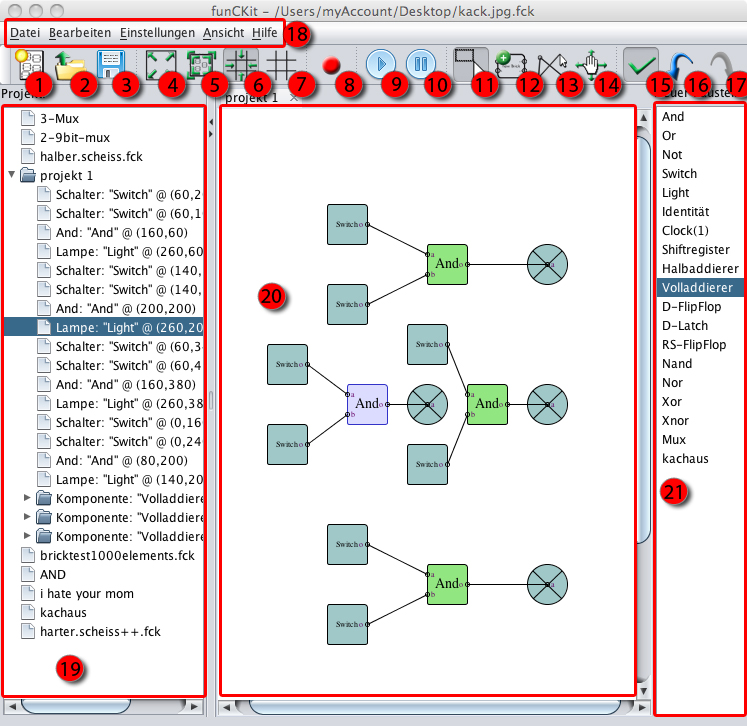
\includegraphics[width=\linewidth]{images/neueBilder/editiermodusNummern.jpg}
	%\caption{?}
\end{figure}

\begin{multicols}{3}
  \begin{itemize}
   \item[1] Neues Projekt
   \item[2] Datei Öffnen
   \item[3] Projekt Speichern
   \item[4] Vollbild
   \item[5] Ansicht einpassen
   \item[6] Gitter einrasten
   \item[7] Gitternetz anzeigen
   \item[8] Simulationshistorie anlegen
   \item[9] Simulation starten
   \item[10] Simulation pausieren
   \item[11] Auswählen/Bewegen
   \item[12] Neues Bauteil
   \item[13] Kabelwerkzeug
   \item[14] Ansicht verschieben
   \item[15] Echtzeitvalidierung
   \item[16] Rückgängig
   \item[17] Wiederherstellen
   \item[18] Menüleiste
   \item[19] Projektbaum
   \item[20] Editierbereich
   \item[21] Neuer Baustein Liste
  \end{itemize}
\end{multicols}

\newpage

\begin{figure}[H]
	\centering
	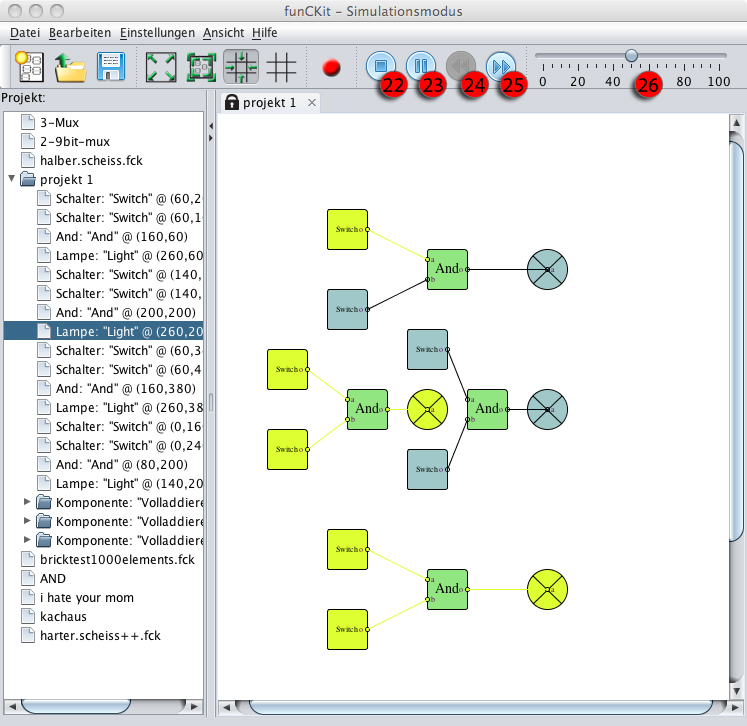
\includegraphics[width=\linewidth]{images/neueBilder/simulationsmodusNummern.jpg}
\end{figure}

\begin{itemize}
  \item[22] Simulation beenden
  \item[23] Simulation Pausieren
  \item[34] Einen Simulationsschritt zurück
  \item[25] Einen Simulationsschritt vorwärts
  \item[26] Simulationsgeschwindigkeit anpassen
\end{itemize}

\subsection{Die Menübar}

\begin{figure}[H]
	\centering
	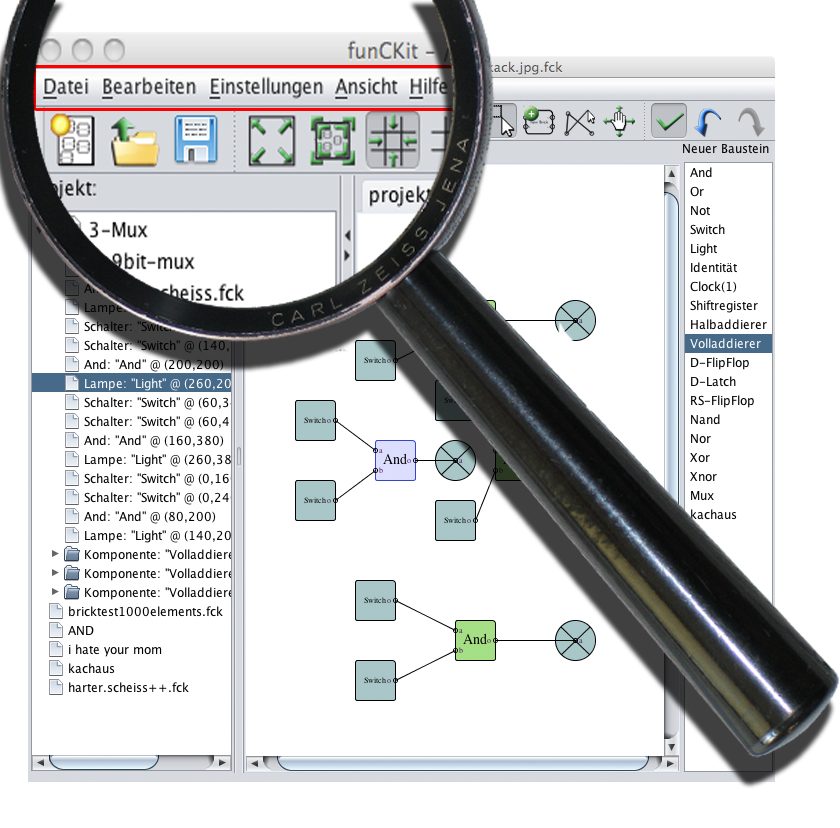
\includegraphics[width=0.6\linewidth]{images/Menuleiste.jpg}
	\label{fig:menubar}
	\caption{Übersicht \fckMenuBar}
\end{figure}
Grundsätzlich teilt sich die Benutzeroberfläche in eine \fckMenuBar, ein \fckEditPanel, einen \fckProjectTree und verschiedene so genannte \fckToolBars - Sammlungen zusammengehörender Werkzeuge.\nlpar
Über die \highlight{\ul{\fckMenuBar}} erreicht man alle wesentlichen Funktionen der Anwendung. Sie teilt sich auf in folgende Punkte:
\begin{enumerate}
	\item \b{Datei} \\
		Menüs mit Verbindung zum Dateisystem oder anwendungsnahe Funktionen. Beispielsweise Anlegen eines neuen Projekts, Speichern und Öffnen von existierenden Projekten oder Import und Export von Komponenten.
		\begin{figure}[H]
			\centering
			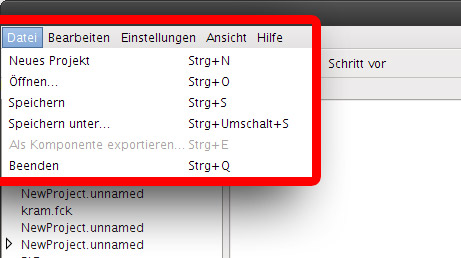
\includegraphics[width=0.6\linewidth]{images/datei.jpg}
			\label{fig:menu-file}
			\caption{Datei Menu}
		\end{figure}
	\item \b{Bearbeiten} \\
		Auswahl von Funktionen, die in Verbindung mit dem Bearbeiten von Schaltungen stehen. Beispielsweise Löschen, Kopieren, Ausschneiden von Bausteinen und Rückgängigmachen von Änderungen.
		\begin{figure}[H]
			\centering
			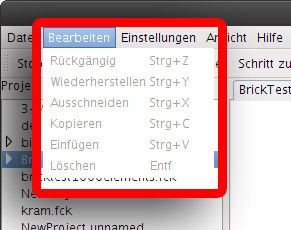
\includegraphics[width=0.5\linewidth]{images/bearbeiten.jpg}
			\label{fig:menu-edit}
			\caption{Bearbeiten Menu}
		\end{figure}
	\item \b{Einstellungen} \\
		Zugriff auf verschiedene Einstellungen wie \fckLiveValidation, Sprache oder Anzeige des Gitternetzes.
		\begin{figure}[H]
			\centering
			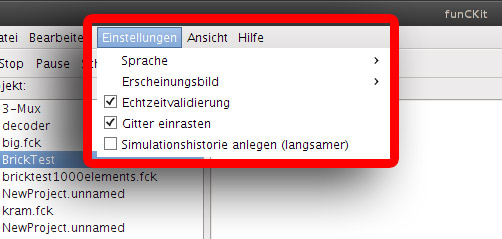
\includegraphics[width=0.6\linewidth]{images/einstellungen.jpg}
			\label{fig:menu-settings}
			\caption{Einstellungen Menu}
		\end{figure}
	\item \b{Ansicht} \\
		Menüpunkt zum Verändern der Ansicht; beispielsweise durch Zoom oder Vollbild.
		\begin{figure}[H]
			\centering
			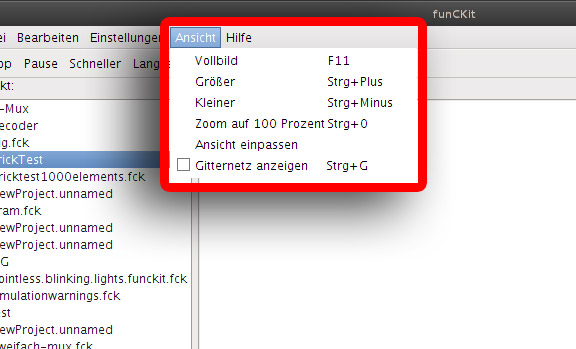
\includegraphics[width=0.7\linewidth]{images/ansicht.jpg}
			\label{fig:menu-view}
			\caption{Ansicht Menu}
		\end{figure}
	\item \b{Hilfe} \\
		Informationen über und zur Verwendung der Anwendung.
		\begin{figure}[H]
			\centering
			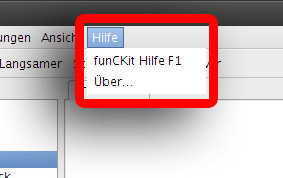
\includegraphics[width=0.5\linewidth]{images/hilfe.jpg}
			\label{fig:menu-help}
			\caption{Hilfe Menu}
		\end{figure}
\end{enumerate}
\vspace{4mm}
Das \highlight{\ul{\fckEditPanel}} ist der zentrale Platz zur Modellierung und Simulation. Es ist je nach Projekt in mehrere \fckTabs (verschiedene Ansichten) angeordnet. Wählt man aus dem \highlight{\fckProjectTree} ein anderes Projekt aus, wechselt man in das \fckEditPanel des entsprechenden Projekts.
\begin{info}
	Über \textit{\gls{cmd-strg-t}} lässt sich ein neuer \fckTab der aktuellen Schaltung öffnen. Damit lässt sich die Schaltung aus mehreren Perspektiven (Zoomstufen, Teilansichten) betrachten. Mit \textit{\gls{cmd-strg-w}} oder mit der mittleren Maustaste auf den Tabnamen lässt er sich wieder schließen.
\end{info} \\
Je nach momentan ausgewähltem \highlight{Tool} kann man verschiedenste Änderungen auf dem Modell vornehmen. Beispielsweise lässt sich über das \highlight{Neues Bauteil }- Tool ein neuer Baustein (Gatter, System- oder eigens definierte Komponente) platzieren oder mit dem \highlight{Auswählen / Bewegen }- Tool bestimmte Bausteine auswählen und verschieben.\nlpar
Um Übersicht über die verschiedenen Projekte zu behalten, gibt es links neben dem Editierfenster angeordnet einen so genannten \highlight{\ul{\fckProjectTree}}. Wird die Anwendung neu gestartet, sind noch keine Projekte vorhanden. Mit zunehmender Verwendung neuer Projekte wächst der \fckProjectTree und man hat schnellen Zugriff auf die jeweiligen Schaltungen. Neben dem Öffnen und der Übersicht vorhandener Projekte, bietet der \fckProjectTree außerdem Einsicht in die verwendeteten Bauteile des Projekts.\nlpar
Neben der \fckMenuBar, dem \fckEditPanel und dem \fckProjectTree existieren außerdem zwei bzw. drei \highlight{\ul{\fckToolBars}}:
\subsection{Editier-Werkzeuge}
Unter der Menüleiste existiert eine Leiste mit verschiedenen Editier-Werkzeugen. Häufig kann man mit einfachen Tastenkürzeln auf andere Editier-Werkzeuge umstellen oder ähnliche Funktionalitäten in verschiedenen Werkzeugen verwenden, so dass eine intuitivere Bedienung möglich ist. Die 4 Editier-Werkzeuge:
\begin{enum}
	\item \b{\fckSelectTool} \\ \\
		{\Large \hspace{0.5em} 
\includegraphics[height=2ex]{images/selecttool.png} \hspace{0.5em}\textbullet \hspace{0.5em} \gls{cmd-strg-1} \hspace{0.5em}\textbullet \hspace{0.5em} \gls{shift}} \\ \\
		Dieses Werkzeug dient dazu, um bereits vorhandene Bausteine und Kabel zu selektieren um diese dann zu verschieben oder zu löschen. Falls zu einer bereits vorhanden Selektion neue hinzugefügt (oder sich bereits in einer Selektion Befindenden entfernt) werden sollen muss die \textit{\gls{cmd-strg}} Taste gedrückt sein. Natürlich gibt es auch das übliche Selektionsviereck, das Sie aus den verschiedensten Programmen kennen. Gelöscht wird mit \textit{\gls{cmd-entf}}, im Menü oder im Kontextmenu. (Rechtsklick) \\
 	\item \b{\fckNewBrickTool} \\ \\
		{\Large \hspace{0.5em} 
\includegraphics[height=2ex]{images/newbricktool.png} \hspace{0.5em}\textbullet \hspace{0.5em} \gls{cmd-strg-2} \hspace{0.5em}\textbullet \hspace{0.5em} \gls{newbricklist}} \\ \\
		Dieses Werkzeug dient dazu, neue Bausteine zu erstellen und schnell unkomplizierte Kabel zu verlegen. Sobald sich sich in diesem Modus befinden erscheint ein sogenannter "Ghostbrick'' im Editpanel, falls der Baustein gezeichnet werden kann. Befindet sich die Maus über einem Accesspoint, so kann mit gedrückter Maustaste die Kabelzeichnung eingeleitet werden. Lässt man über einem anderen Accesspoint die Maustaste wieder aus, so werden diese beiden Punkte mit einem Kabel verbunden. Macht man das Selbe jedoch an "freier Stelle'', so springt das Programm automatisch ins Wiretool. \\
	\item \b{\fckWireTool} \\ \\
		{\Large \hspace{0.5em} 
\includegraphics[height=2ex]{images/wiretool.png} \hspace{0.5em}\textbullet \hspace{0.5em} \gls{cmd-strg-3}} \\ \\
		(Erreichbarkeit fehlt: button, alle kürzel)
		Mit diesem Werkzeug können ganz frei Kabel gezeichnet werden. Befindet man sich in diesem Modus, so kann an beliebiger Stelle mit dem Zeichnen eines Kabels begonnen werden, indem an beliebiger Stelle geklickt wird. Man kann auch an bestehende Kabel und Accesspoints anknüpfen. Es muss beachtet werden, dass sich anfangs erst um sogannte ``GhostWires'' handelt. Mit \textit{\gls{cmd-esc}} oder Rechtsklick kann das ``GhostWires'' wieder entfernt werden. Mit einem einfachen Klick auf einen Accesspoint oder Doppelklick auf eine freie Fläche wird das Kabel befestigt und funktionsfähig. \\
	\item \b{\fckMoveViewportTool} \\ \\
		{\Large \hspace{0.5em} 
\includegraphics[height=2ex]{images/moveviewporttool.png} \hspace{0.5em}\textbullet \hspace{0.5em} \gls{cmd-strg-4} \hspace{0.5em}\textbullet \hspace{0.5em} \gls{space}} \\ \\
		Mit diesem Werkzeug können sie sich leicht sehr schnell über die gesamte Schaltung (und darüber hinaus) bewegen. \\
\end{enum}

\begin{info}
	Mit \textit{\gls{cmd-strg-1}}, \textit{\gls{cmd-strg-2}}, \textit{\gls{cmd-strg-3}} und \textit{\gls{cmd-strg-4}} lässt sich ganz einfach zwischen den wichtigsten Tools (\textit{\fckSelectTool, \fckNewBrickTool, \fckWireTool} und \textit{\fckMoveViewportTool}) hin- und herwechseln.
\end{info}

\subsection{\fckNewBrickList}
		\setlength{\intextsep}{0pt}
		\begin{wrapfigure}{r}{1.8cm}
		      \centering
		      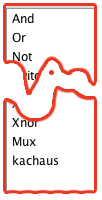
\includegraphics[width=1.8cm]{images/neueBilder/blicklist.png}
		\end{wrapfigure}
		Die \fckNewBrickList dient zur Übersicht von existierenden Bausteinen, die in der aktuellen Schaltung hinzugefügt werden können. Sie beinhaltet sowohl grundlegende Gatter wie \textit{And}, \textit{Or} und \textit{Not}, vorgegebene Systemkomponenten (\textit{XOR} oder \textit{NOR}), als auch eigens über den Export definierte Komponenten - worüber man eine ganze Reihe komplexerer Bausteine leicht hinzufügen kann (beispielsweise selbst gestaltete arithmetisch-logische Einheiten). Durch Klicken auf eines dieser Bricks wechseln sie in das ``New-Brick-Tool''.
\subsection{Simulationsbedienung}
                {\Large \hspace{0.5em} 
\includegraphics[height=2ex]{images/control_play_blue.png} \hspace{0.5em}   
\includegraphics[height=2ex]{images/control_pause_blue.png} \hspace{0.5em}   
\includegraphics[height=2ex]{images/control_rewind_blue.png}  \hspace{0.5em} 
\includegraphics[height=2ex]{images/control_rewind_blue_TURNED.png} } \\ \\
		Startet man aus dem Editieren heraus die Simulation, verschwinden die Editier-Werkzeuge und die Steuerungsleiste zur Simulation tritt an ihre Stelle. Über diese \fckToolBar lässt sich die Simulation pausieren, beschleunigen, verlangsamen oder schrittweise voranschreiten. Wenn die Simulationshistorie auch aktiviert ist, lässt sich die Simulation sogar schrittweise zurücksetzen.

% Einführung ins Bearbeiten von Schaltungen
\subsection{Editieren}
		\begin{figure}[H]
			\centering
			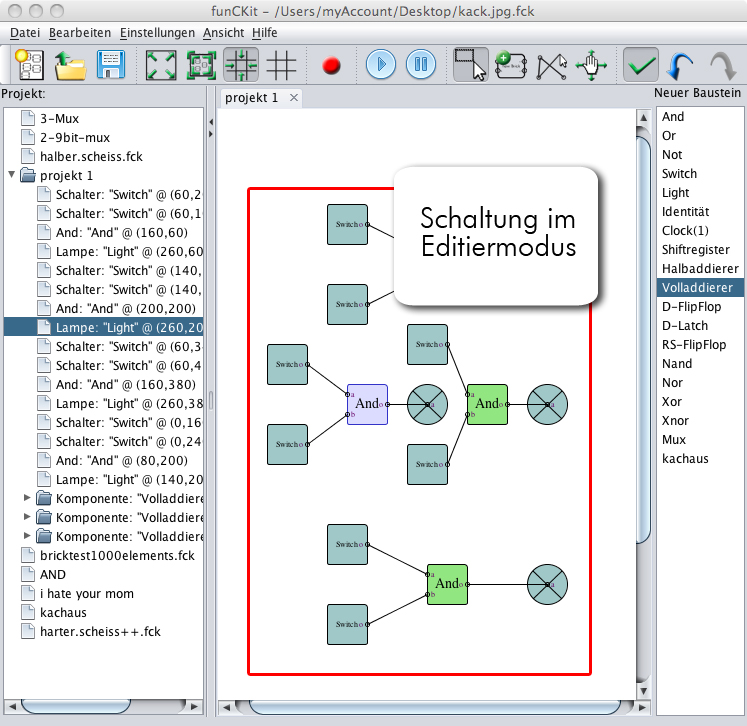
\includegraphics[width=\linewidth]{images/schaltungImEditiermodus.jpg}
			\label{fig:circuit-editmode}
			\caption{Editiermodus}
		\end{figure}
In diesem Abschnitt wird das wesentliche Bearbeiten einer Schaltung erläutert - beginnend beim Anlegen eines Projekts über Hinzufügen und Verknüpfen und bis hin zum Entfernen und Bearbeiten von Bausteinen. Daneben werden einige praktische Funktionalitäten beim Editieren erwähnt, auf die im Abschnitt ">\textit{Features im Detail}"< näher eingegangen wird.
\subsubsection{Neues Projekt}
{\Large \hspace{0.5em} 
\includegraphics[height=2ex]{images/newProject.png} \hspace{0.5em}\textbullet \hspace{0.5em} \gls{cmd-strg-n} } \\ \\
Nach dem ersten Start der Anwendung existieren noch keinerlei Projekte im Projektbaum. Man kann also entweder ein neues (leeres) Projekt anlegen oder eine bestehende Schaltung öffnen bzw. importieren. Auf Import und Export wird später detaillierter eingegangen. Für ein neues Projekt reicht zu Beginn ein Projektname aus. So lange nicht gespeichert wurde, existiert das Projekt nur temporär.
\begin{info}
	Mit den Tastenkombinationen \textit{\gls{cmd-strg-s}} bzw. \textit{\gls{cmd-strg-shift-s}} lässt sich ein Projekt schnell speichern bzw. unter einem neuen Ort speichern.
\end{info} \\
Nach dem Erstellen des Projekts, erscheinen nun die Editier-Werkzeuge und eine \fckNewBrickList. Außerdem hält der Projektbaum nun das neue Projekt vor und lässt sich nach dem Speichern darüber immer wieder neu laden. Über ">Ansicht $\ra$"< Gitter anzeigen (oder \textit{\gls{cmd-strg-g}}) lässt sich übrigens ein Hilfsgitter im Hintergrund anzeigen.
\subsubsection{Bausteine erstellen}
		\begin{figure}[H]
			\centering
			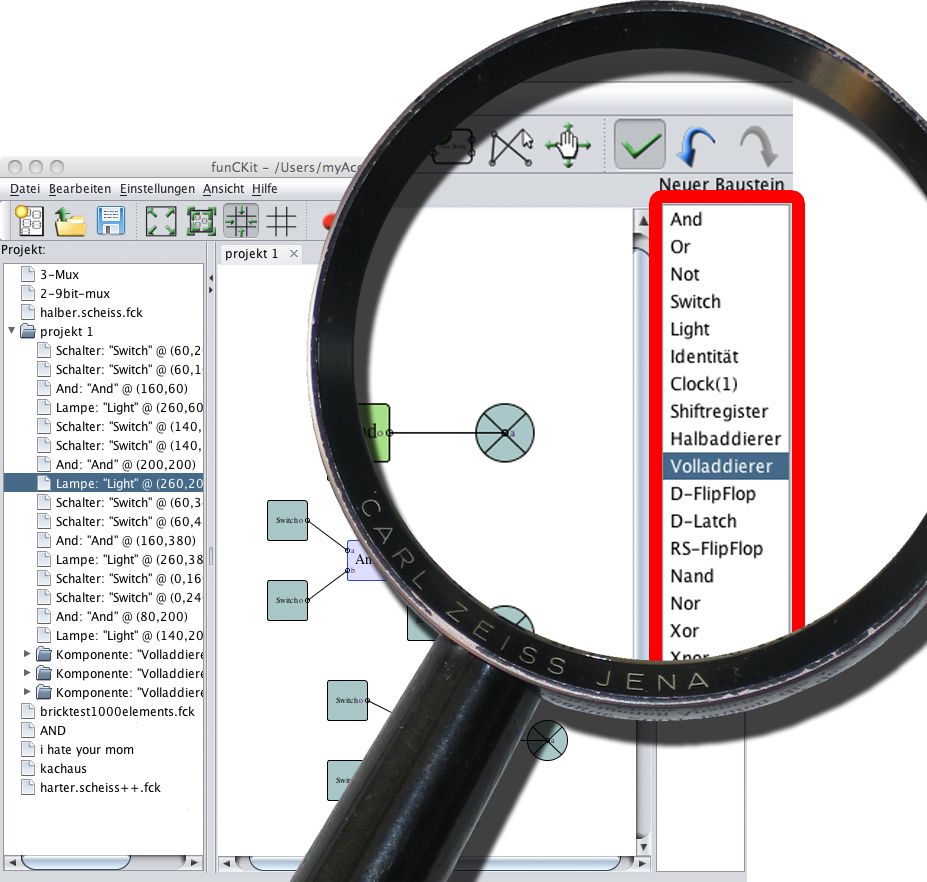
\includegraphics[width=0.5\linewidth]{images/NeuerBausteinListe.jpg}
			\label{fig:new-brick-list}
			\caption{Neuer Baustein Liste}
		\end{figure}
Über die \highlight{Neue Baustein - Liste }lässt sich nun ein Bausteintyp auswählen und auf dem Editierfenster platzieren. Überschneidungen werden grundsätzlich vermieden, auch wenn die Anwendung grundsätzlich damit arbeiten kann (einige Exportformate unterstützen keine Überschneidung von Bausteinen). Über die Einstellungen kann man zusätzlich ``Gitter einrasten'' aktivieren und damit sauberere Entwürfe anlegen.
\subsubsection{Bausteine verbinden}
Kabelverbindungen lassen sich entweder aus dem \textit{\fckNewBrickTool} heraus direkt oder ausführlicher mit dem \textit{\fckWireTool} erstellen. Eine Verbindung kann von einem beliebigen Verbindungspunkt an einem Baustein zu einem anderen Verbindungspunkt verlaufen. Dabei ist es zunächst nicht relevant ob es sich dabei um Ein- oder Ausgänge handelt.
\begin{info}
	Unter ">Einstellungen $\ra$ Echtzeitvalidierung"< lässt sich eine automatische Validierung der aktuellen Schaltung aktivieren. Damit werden sofort Bereiche der Schaltungen markiert, die für einen fehlerhaften Graphen verantwortlich sind und damit nicht simuliert werden können.
\end{info} \\
Um eine korrekte (= simulierbare) Schaltung zu modellieren, müssen Verbindungen von Ausgängen zu Eingängen führen. Bei welchem Verbindungspunkt man startet, ist dabei aber egal. Aus dem \textit{\fckNewBrickTool} kann man mit Hilfe eines haltenden Klicks auf einen Verbindungspunkt und Ziehen des angezeigten Kabels eine Verbindung zu einem anderen Baustein herstellen. Lässt man das Kabel an einer freien Stelle im Modell los, wechselt man automatisch in das \textit{\fckWireTool} und kann mit einer Verzweigung die Verbindung an dieser Stelle fortsetzen.

Im \textit{\fckWireTool} reicht ein einfacher Klick auf den Verbindungspunkt, um das Anlegen einer Verbindung zu starten. Klicks auf freie Flächen erzeugen Verbindungspunkte, an denen man die Verbindung verzweigen oder umknicken lassen kann. Doppelklicks ermöglichen es, die Verbindung an dieser Stelle zu beenden und das Kabel an einem Verbindungspunkt enden zu lassen. Mit einem Klick auf einen anderen Verbindungspunkt wird das Erstellen der Verbindung abgeschlossen.

Hat man aus dem \textit{\fckNewBrickTool} heraus begonnen eine Verbindung zu erstellen, wechselt man nach Abschließen der Verbindung zurück in diesen Modus. Andernfalls kann man direkt im \textit{Kabel - Werkzeug} weitere Verbindungen zwischen Bausteinen erstellen.
\begin{info}
	Hat man einmal einen falschen Verbindungspunkt ausgewählt, kann man die aktuelle Verbindung mit \textit{Esc} abbrechen. Außerdem lässt sich über \textit{\gls{cmd-strg-z}} eine Änderung rückgängig machen und mit Hilfe von \textit{\gls{cmd-strg-y}} wiederherstellen.
\end{info}

\subsubsection{Bearbeiten der Schaltung}
Mit dem Erstellen und Verbinden von Bausteinen kann man bereits eine größere Schaltung entwerfen. Oft fällt während dem Editieren aber auf, dass sich Fehler eingeschlichen haben, oder Umordnungen sinnvoll wären. Dazu kann man die erstellen Elemente mit Hilfe verschiedener Möglichkeiten wieder bearbeiten.

Über den \highlight{Selektionsmodus }(\textit{\gls{cmd-strg-1}}) lassen sich ein oder mehrere Elemente auf der Schaltung auswählen. Ausgewählte Elemente können verschoben, gelöscht, kopiert und sogar zwischen verschiedenen Projekten ausgetauscht werden. Dazu dienen verschiedene Funktionen, die sich über die Menüleiste oder durch Tastenkombinationen erreichen lassen.

Am einfachsten lassen sich bereits erstellte Bausteine über die \textit{Entf}-Taste wieder löschen. Der entsprechende Menüpunkt dazu befindet sich unter ">Bearbeiten $\ra$ Löschen"<.

Ausgewählte Elemente können durch Ziehen und wieder Loslassen der Maus verschoben werden. So genannte \textit{Geist-Elemente} helfen bei der exakten Positionierung der zu verschiebenden Elemente.
\begin{info}
	\b{Komfort vs. Einbußen:} Verbindungspunkte haben beim Erstellen von Verbindungen einen so genannten \textit{Toleranzbereich}. Dieser Toleranzbereich dient dazu, dass man Verbindungspunkte nicht exakt treffen muss, um eine neue Verbindung von einem Baustein zu einem anderen zu erstellen (oder gar eine längere Verbindungsreihe mit vielen weiteren Verbindungspunkten).
	Der Komfort hat aber einige Einbußen, so dass man keine Verbindungen ganz nah an einen Verbindungspunkt setzen kann, ohne die beiden zu verknüpfen. \\
	\b{Die Lösung:} Man setzt eine Verbindung etwas daneben und kann mit dem Selektionswerkzeug Verbindungspunkte eines Kabels ganz einfach verschieben.
\end{info}

\subsection{Komponenten}
Komponenten sind selbst definierte Bausteine, die wiederum aus Bausteinen bestehen und sich somit auf die grundlegenden Gatter \textit{And}, \textit{Or} und \textit{Not} runterbrechen lassen. Sobald man eigene Komponenten definiert hat, kann man so sehr einfach Übersicht in seiner Schaltung schaffen.

\subsubsection{Systemkomponenten}
Systemkomponenten unterscheiden sich von den restlichen Komponenten insoweit, dass sie bereits mit der Anwendung mitgeliefert werden. Je nach Version können das unterschiedlich viele sein. Beispielhafte Systemkomponenten sind \textit{Nand}-, \textit{Nor}-, \textit{Xor}-Gatter oder \textit{Clocks}.

\subsubsection{Komponenten erstellen}
In \projectName können Schaltungen als Komponenten exportiert werden, indem alle Schalter als Eingänge und alle Lichter als Ausgänge der Komponente verwendet werden. Die Reihenfolge der generierten Ein- und Ausgänge richtet sich hierbei nach der vertikalen Position der Schalter bzw. Lichter. Diesem Schema entsprechend werden die Namen der Schalter und Lichter als namen der Ein- bzw Ausgänge übernommen.

Zum exportieren dieser so erstellten Schaltung, wählt man im Menü Datei den Punkt \textsl{Als Komponente Exportieren}. Wird die Komponente im vorgegebenen Pfad gespeichert taucht sie in der \fckNewBrickList auf und kann verwendet werden.

\subsubsection{Komponenten bearbeiten}
Komponenten können über \textsl{Datei \textrightarrow Öffnen...} importiert und dann auf gewöhnliche Art und Weise bearbeitet werden.

\subsubsection{in Komponenten hineinschauen}
Um besser nachvollziehen zu können, was im Inneren einer Komponente passiert öffnet sich bei Doppelklick darauf einer neuer Tab mit dem Aufbau der Komponente. Hier kann nichts editiert werden, deshalb befindet sich am Register auch das Schloss.

\subsubsection{Komponenten als neues Projekt öffnen}
,Damit schnell und einfach bestehende Komponenten als Vorlage für eine neue Schaltung oder für eine eine neue Komponente zur Verfügung stehen, kann man diese durch rechtsklick auf der Komponente oder im Komponentenbaum als neues Projekt öffnen.


% Einführung in die Simulationsbedienung und die Möglichkeiten während der Simulation die Zustände zu beobachten
\subsection{Simulieren}
		\begin{figure}[H]
			\centering
			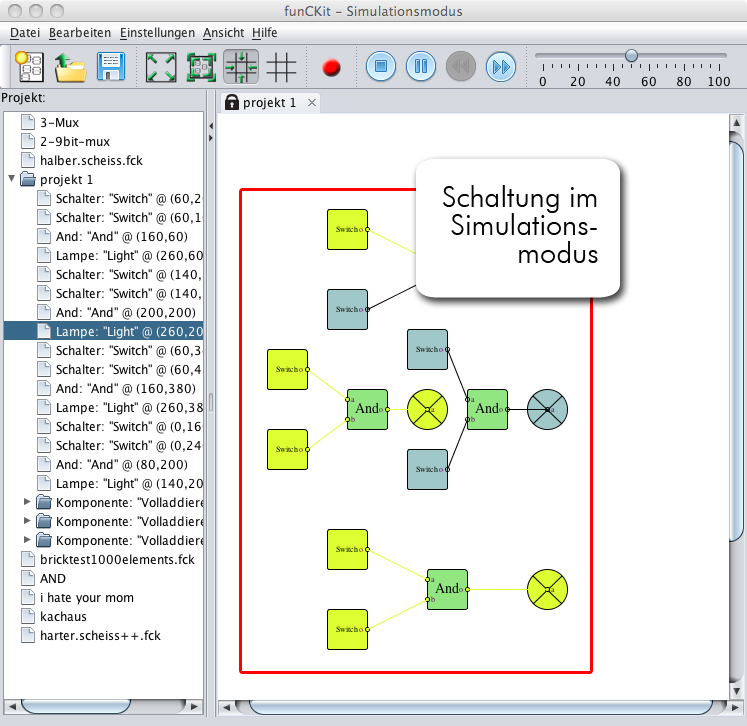
\includegraphics[width=\linewidth]{images/simulationsmodus.jpg}
			\label{fig:circuit-simulationmode}
			\caption{Simulation}
		\end{figure}
Aus dem Editiermodus heraus lässt sich mit dem Simulations-Startknopf eine Simulation der aktuell geöffneten Schaltung starten. Während der Simulation kann man auf ein anderes Projekt (und damit eine andere Schaltung) wechseln, wodurch die aktuelle Simulation pausiert. So können parallel auch mehrere Simulationen gestartet werden.

Die Simulation startet nur, wenn die Validierung zur Simulation erfolgreich war. Diese Validierung prüft auf notwendige Eigenschaften, die die Schaltung erfüllen muss. Beispielsweise dürfen keine Rückkopplungen (Schleifen) ohne Verzögerung stattfinden. Eine entsprechende Fehlermeldung wird angezeigt.
\begin{info}
	Echtzeitvalidierung kann während der Modellierung bereits dabei helfen, Fehler in der Schaltung zu finden und sie so simulierbar zu halten, um manuell den logischen Ablauf der modellierten Schaltung zu überprüfen.
\end{info} \\
In der Simulation selbst werden - im näheren Zoom auf die Schaltung - Leitungen und Lampen als aktiv oder inaktiv markiert (\textit{logisch-0} und \textit{logisch-1}). Die drei Grundgatter \textit{And}, \textit{Or} und \textit{Not} können auch je nach Verzögerungszahl ihre anliegende Queue für jeden Ausgang anzeigen (wird bei aktivem Hervorheben mit der Maus über dem Baustein sichtbar).

Über die Werkzeuge in der Simulations-Werkzeugleiste kann man die Geschwindigkeit der Simulation verändern oder schrittweise die Simulation voranschreiten lassen, um einzelne Zustandsveränderungen detaillierter beobachten zu können.

Wenn ">Einstellungen $\ra$ Simulationshistorie anlegen"< aktiviert ist, kann die Simulation auch schrittweise rückwärts gegangen werden (sofern bereits entsprechende Simulationsschritte ausgeführt wurden). Die Simulationshistorie wird sowohl in der automatischen (geschwindigkeitsgeregelten), als auch in der schrittweisen Simulation angelegt.
\begin{info}
	\b{Komfort vs. Einbußen:} Zwar ist es durchaus vorteilhaft zum debuggen, aber während der Simulation eine Historie mitlaufen zu lassen, kostet deutlich mehr Rechenleistung, als wenn ohne Zustandskopie simuliert wird. Das hat den Grund, dass für jeden Simulationsschritt der Gesamtzustand der Simulation gespeichert werden muss. Somit ist eine flüssige Darstellung der Simulation ggf. nicht mehr möglich. \\
	\b{Die Lösung:} Sinnvoll ist es bis zu bestimmten Zuständen ``hin'' zu simulieren, um dann erst schrittweise mit Simulationshistorie fehlerhaftes Verhalten der Schaltung zu untersuchen. Durch regelmäßiges Aktivieren \& Deaktivieren verhindert man verzögerte Reaktionen.
\end{info}


\subsection{Speichern und Öffnen}
\subsubsection{Speichern}

		{\Large \hspace{0.5em} 
\includegraphics[height=2ex]{images/disk.png} \hspace{0.5em}\textbullet \hspace{0.5em} \gls{cmd-strg-s} \hspace{0.5em}} \\ \\
Zum Speichern des aktuell geöffneten Projektes wählen Sie ">Datei $\ra$ Speichern"< oder drücken Sie \gls{cmd-strg-s}. Sollten Sie ein Windows oder Mac Betriebssystem verwenden, so wird der Dateityp über die eingegebene Dateiendung bestimmt. Andernfalls können Sie diesen über den \fckOpenDialog wählen. Zur Speicherung wird das \projectName Dateiformat empfohlen. Zur Auswahl stehen zum einen einige Bildformate (PDF, PNG, GIF, SVG, JPG), zum anderen das \fckSEPFormat. Die Speicherung im \fckSEPFormat wird ausdrücklich nicht empfohlen, da aufgrund der Einschränkungen des Formates nicht der volle Funktionsumfang gewährleistet werden kann. So ist es nicht möglich Schaltungen zu speichern, in denen Bausteine an der selben Position platziert wurden.

\subsubsection{Öffnen}

		{\Large \hspace{0.5em} 
\includegraphics[height=2ex]{images/open.png} \hspace{0.5em}\textbullet \hspace{0.5em} \gls{cmd-strg-o} \hspace{0.5em}} \\ \\
Zum Öffnen eines Projektes wählen Sie ">Datei $\ra$ Öffnen"< oder drücken Sie \gls{cmd-strg-o}. Wählen Sie nun die gewünschte Datei aus und drücken Sie \textit{Öffnen}. Während die Datei geladen wird, präsentiert sich Ihnen eine Fortschrittsanzeige und Sie haben die Möglichkeit, den Vorgang abzubrechen. War das Laden erfolgreich, so wird das Projekt in den Projektbaum aufgenommen und eine Ansicht der Hauptschaltung geöffnet.

% Umgang mit Fehlern auf der Oberfläche (Neustarts, Backups, ..)
%\subsection{Fehlerbehandlung}
%-
%\subsubsection{Einstellungen manuell bearbeiten}
%-


% 
% Umfangreiche Beschreibung der Funktionalitäten ohne größeren Zusammenhang. Unterscheidet sich von der Bedienungsanleitung also insofern, dass kein schrittweiser, sondern
% ein struktureller Aufbau stattfindet.
%
\section{Features im Detail}
\subsection{Tools}
Die Software stellt viele nützliche Tools zur leichteren Bedienung des Programms zur Verfügung, damit schnell und einfach Schaltungen erzeugt werden können. Diese Tools werden im Folgenden aufgelistet:
\begin{enum}
	\item \textbf{\fckSelectTool} \\
		Mit Hilfe dieses Tools lassen sich Linien, Gatter und Komponenten markieren und diese zu dem gewünschten Platz im Gitternetz ziehen. Dabei wird das markierte Element beim Verschieben zur besseren Orientierung im Fenster grau gezeichnet. \\
		Über \textit{\gls{cmd-strg-a}} werden alle Elemente im Editierfenster markiert. Des weiteren ist es möglich, markierte Elemente mit Hilfe von \textit{\gls{cmd-strg-c}} zu kopieren und diese über \textit{\gls{cmd-strg-v}} wieder am gewünschten Ort einzufügen. \\
		Kopierte Elemente können bei jedem geöffnetem Projekt einfügt werden.
	\item \textbf{\fckNewBrickTool} \\
		Durch das \textit{\fckNewBrickTool}  wählt man aus der \textit{\fckNewBrickList} das gewünschte Gatter aus, z.B. \textit{And-Gatter} oder vordefinierte Komponenten(u.a. \textit{Xor}, \textit{Nand}), und platziert diese im Gitternetz. In diesem Modus ist es außerdem möglich, einzelne Gatter untereinander durch Linien zu verbinden.
	\item \textbf{\fckWireTool} \\
		Im \textit{Neuen-Baustein-Modus} lassen sich Gatter untereinander verbinden. Mit Hilfe des \fckWireTool lassen sich jedoch auch Gatter verbinden, aber im diesem Modus können zur Übersichtlichkeit der Schaltung Verbindungen um Gatter herum platzieren werden. Klickt man auf einen Eingang bzw. Ausgang eines Gatters, erscheint der Anfangspunkt der Verbindung. Um jetzt zwei Gatter miteinander zu verknüpfen, können Wegpunkte für die Verbindung bei Mausklick im Gitternetz gesetzt werden. \\
		Schließlich werden die gewünschten Gatter miteinander verbunden. \\
		Mit diesem Tool ist es des weiteren möglich, Verzweigungen von Verbindungen zu machen. Dazu klickt man einfach auf die Verbindung (es wird ein Verzweigungspunkt gesetzt), und verfolgt den gleichen Schritt wie zu Beginn.
	\item \textbf{\fckMoveViewportTool} \\
		Mit gedrückter Maustaste lässt sich in diesem Modus das Editierfenster zum gewünschten Bereich verschieben. \\
		Unter ">\textit{Ansicht} $\ra$ \textit{Ansicht anpassen}"< wird das Editierfenster der Schaltung angepasst, damit alle Elemente darin sichtbar werden.
\end{enum}
\begin{info}
	Mit \textit{\gls{cmd-space}} + linke Maustaste lässt sich die Anzeige aus jedem Tool heraus bequem verschieben ohne in den \textit{Ansicht verschieben - Modus} wechseln zu müssen.
\end{info}


%\subsection{Komponenten verwalten}
%-
\subsection{Der Projektbaum}
Der Projektbaum dient der Verwaltung der bekannten \glspl{Projekt} sowie zur Navigation zwischen den geöffneten Projekten. 

\subsubsection{Verwaltung von Projekten}
  Auf der obersten Ebene des Baumes sind die der Anwendung bekannten \glspl{Projekt} Aufgelistet. Hierbei sind geöffnete (ausklappbar) und geschlossene \glspl{Projekt} zu unterscheiden. 

  \begin{info}
        Geschlossene \glspl{Projekt} können durch einen Doppelklick geöffnet werden.
  \end{info}

  Durch markieren eines einzelenen (geöffneten) \gls{Projekt}es wird in dieses gewechselt. Beim Rechtsklick auf ein (geöffnetes) \glspl{Projekt} erscheint ein Kontextmenü mit folgenden Optionen:
  \begin{itemize}
  \item \textbf{In einem neuen Reiter öffnen} \\
      Öffnet eine neue Ansicht der Hauptschaltung des Projektes in einem neuen Reiter.  
  \item \textbf{Projekt schließen} \\
      Schließt das Projekt.
  \item \textbf{Projekt löschen} \\
      Löscht das Projekt aus dem Projektbaum. Eine eventuell zugehörige Datei bleibt erhalten so dass das Projekt über den \fckOpenDialog wieder geladen werden kann.
  \item \textbf{Projektnamen ändern} \\
      Ermöglicht es den Projektnamen zu ändern.
  \end{itemize}

\subsection{Navigation innerhalb von Projekten}
Durch aufklappen eines Projektes im Baum erhält man eine Auflistung aller Bausteine innerhalb der Hauptschaltung mit Typ, Name und Position innerhalb der Schaltung. Ein markieren eines dieser Baustein-Einträge bewirkt, dass der entsprechende Baustein innerhalb des Anzeigebereichs der Schaltung markiert und dieser innerhalb des Anzeigebereichs zentriert wird. Das Kontextmenü bietet hier folgende Operationen:
\begin{itemize}
	\item \textbf{Baustein löschen} \\
		Löscht den zugehörigen Baustein aus der Schaltung.
	\item \textbf{Eigenschaften} \\
		Zeigt den Einstellungsdialog des zugehörigen Bausteins an in dem dessen Name, Größe und ähnliches verändert werden können.
\end{itemize}
\noindent Eine besondere Rolle nehmen die Einträge für Bausteine vom Typ ``Komponente'' ein. Diese lassen sich widerum aufklappen. Hier wird dann der Typ der Komponente angezeigt (z.B. ``SHIFTREGISTER''), der widerum aufgeklappt werden kann und den Inhalt der \gls{Schaltung} der Komponente auflistet. Bei Komponenten bietet das Kontextmenü folgende weitere Optionen:
\begin{itemize}
	\item \textbf{In einem neuen Reiter öffnen} \\
		Öffnet eine Ansicht der Komponente in einem neuen Reiter.
	\item \textbf{Als neues Projekt öffnen} \\
		Erstellt ein neues Projekt mit der Schaltung des Komponententyps als Hauptschaltung.
\end{itemize}


\subsection{Einstellungen}
  Im Menüpunkt \textsl{Einstellungen} können zahlreiche Einstellungen am Programm vorgenommen werden. Diese Einstellungen werden in einer Konfigurationsdatei abgespeichert und bleiben auch nach dem Neustart des Programmes erhalten. Im folgenden sind dies:
  \begin{itemize}
   \item \textbf{Sprache} \\
      Hier kann eine der Sprachen ausgewählt werden, in die das programm übersetzt ist. Diese Einstellung wird erst nach einem Neustart des Programmes wirksam, in dem alle ungespeicherten Änderungen verloren gehen.
   \item \textbf{Erscheinungsbild} \\
      Hier kann das Erscheinungsbild der Anwendung verändert werden. Diese Einstellung wird erst nach einem Neustart des Programmes wirksam, in dem alle ungespeicherten Änderungen verloren gehen.
   \item \textbf{Echtzeitvalidierung} \\
	{\Large \hspace{0.5em} 
\includegraphics[height=2ex]{images/livecheck.png} \hspace{0.5em}}
      Hier kann die Echtzeitvalidierung ein bzw. ausgeschaltet werden, da diese sehr aufwendig ist und beim bearbeiten von größeren Schaltungen zu unerwünschten Verzögerungen führen kann.
   \item \textbf{Gitter Einrasten} \\
	{\Large \hspace{0.5em} 
\includegraphics[height=2ex]{images/gridlock.png} \hspace{0.5em}}
      Hier kann man einstellen, ob beim erstellen oder Verschieben von Bausteinen diese am Gitternetz einrasten sollen oder nicht.
   \item \textbf{Simulationshistorie anlegen} \\
	{\Large \hspace{0.5em} 
\includegraphics[height=2ex]{images/record.png} \hspace{0.5em}}
      Hier kann man festlegen, ob eine Historie der Simulation angelegt werden soll. Dies ermöglicht ein Rückwärtslaufen der Simulation, verlangsamt diese aber.
   \item \textbf{Niedrige Qualität} \\
      Hier kann auf eine niedrigere Anzeigequalität gewechselt werden. Die kann gerade bei größeren Schaltungen ein flüssigeres Arbeiten ermöglichen.
   \item \textbf{Tooltips Ein/Aus} \\
      Stellt ein, ob die \glspl{Tooltip}s für Bauteile der Schaltung angezeigt werden sollen oder nicht.
   \item \textbf{Standardeinstellugnen wiederherstellen} \\
      Stellt die Standardeinstellungen wieder her.
  \end{itemize}


\subsection{Shortcuts}
Die Tastaturbelegungen zur leichteren Bedienung der Software in Übersicht:
\begin{enum}
	\item \textbf{Datei}
		\begin{enum}
			\item \textit{\gls{cmd-strg-n}}: Neues Projekt anlegen
			\item \textit{\gls{cmd-strg-o}}: Gespeichertes Projekt öffnen
			\item \textit{\gls{cmd-strg-s}}: Projekt speichern
			\item \textit{\gls{cmd-strg-shift-s}}: Projekt speichern unter
			\item \textit{\gls{cmd-strg-e}}: Komponente exportieren
			\item \textit{\gls{cmd-strg-q}}: Programm beenden
		\end{enum}
\end{enum}
\begin{enum}
	\item \textbf{Bearbeiten}
		\begin{enum}
			\item \textit{\gls{cmd-strg-z}}: Rückgänging machen
			\item \textit{\gls{cmd-strg-y}}: Wiederherstellen
			\item \textit{\gls{cmd-strg-x}}: Ausschneiden
			\item \textit{\gls{cmd-strg-c}}: Kopieren
			\item \textit{\gls{cmd-strg-v}}: Einfügen
			\item \textit{\gls{cmd-entf}}: Löschen
		\end{enum}
\end{enum}
\begin{enum}
	\item \textbf{Ansicht}
		\begin{enum}
			\item \textit{\gls{cmd-f11}}: Vollbild
			\item \textit{\gls{cmd-strg-plus}}: Größer (nicht bei Mac OS X)
			\item \textit{\gls{cmd-strg-minus}}: Kleiner (nicht bei Mac OS X)
			\item \textit{\gls{cmd-strg-0}}: Zoom auf 100-Prozent
			\item \textit{\gls{cmd-strg-g}}: Gitternetz anzeigen
		\end{enum}
\end{enum}
\begin{enum}
	\item \textbf{Hilfe}
		\begin{enum}
			\item \textit{\gls{cmd-f1}}: \projectName Hilfe
		\end{enum}
\end{enum}
\begin{enum}
	\item \textbf{Editieren}
		\begin{enum}
			\item \textit{\gls{cmd-strg-1}}: \fckSelectTool
			\item \textit{\gls{cmd-strg-2}}: \fckNewBrickTool
			\item \textit{\gls{cmd-strg-3}}: \fckWireTool
			\item \textit{\gls{cmd-strg-4}} oder \textit{\gls{cmd-space}} + linke Maustaste: \fckMoveViewportTool
			\item \textit{\gls{cmd-strg-t}}: Neuer Tab
			\item \textit{\gls{cmd-strg-w}} oder mittlere Maustaste: Tab schließen
		\end{enum}
\end{enum}
\begin{enum}
	\item \textbf{Bedienung}
		\begin{enum}
			\item \textit{\gls{cmd-scroll}}: scrollen
			\item \textit{\gls{cmd-strg-scroll}}: zoomen
			\item \textit{\gls{cmd-alt-scroll}}: horizontal scrollen
		\end{enum}
\end{enum}

%
% Beschreibung vom Dateiformat
%
\newpage
\appendix
\section{Dateiformat}
Das von \projectName verwendete Dateiformat stellt eine Abwandlung des \fckSEPFormatGenitive dar und baut auf der Extensible Stylesheet Language\footnote{\url{http://www.w3.org/TR/2008/REC-xml-20081126/}} auf.

\subsection{Anforderungen} 
Um eine Datei im \fckSEPFormat als \projectName-Datei zu Kennzeichnen, muss der zugehörige Namespace ``\textit{fck}'' verwendet werden. Dazu ist im Tag ``\textit{circuits}'' {
	\center{\textbf{xmlns:fck=``http://git.sep2011.de/funckit''}} \\
}
\noindent zu setzen. Jede so markierte Datei kann nur geladen werden wenn sie sämtliche der nachfolgenden Anforderungen erfüllt:
\begin{enum}
	\item \textbf{circuits} \\
		Das Element \textit{circuits} muss das Attribut \textit{fck:projectname} enthalten.
	\item \textbf{circuit} \\
		Sofern das Attribut \textit{fck:type} auf \textit{component} gesetzt ist müssen die Attribute \textit{fck:height}, \textit{fck:name}, \textit{fck:orientation} und \textit{fck:width} vorhanden sein.
	\item \textbf{component} \\
		Eine \textit{component} muss die Attribute \textit{fck:height}, \textit{fck:name}, \textit{fck:orientation} und \textit{fck:width} enthalten. Desweiteren müssen, falls es sich um den \textit{type} \textit{circuit} handelt, die Elemente \textit{accesspoint} und \textit{mapping} jeweils paarweise enthalten sein. Dabei müssen die \textit{fck:id} und \textit{fck:outerPoint} Attribute übereinstimmen. Das \textit{fck:innerPoint} Attribut muss dabei das \textit{name} Attribut einer \textit{component} in der duch \textit{type2} referenzierten \textit{circuit} deren Attribut \textit{fck:componentTypePoint} auf \textit{true} gesetzt ist referenzieren. \\
		Hat eine \textit{component} das Attribut \textit{fck:componentTypePoint} auf \textit{true} gesetzt, so darf es nur die Attribute \textit{fck:name}, \textit{fck:posx} und \textit{fck:posy} enthalten. \\
		Eine \textit{component} kann das Attribut \textit{fck:delay} enthalten, sowie Elemente vom Typ \textit{accesspoint}.
	\item \textbf{connection} \\
		Eine \textit{connection} muss, sofern nicht das Attribut \textit{fck:ignore} auf \textit{true} gesetzt ist, die Attribute \textit{fck:name}, \textit{fck:source} und \textit{fck:target} enthalten. Dabei müssen \textit{fck:source} und \textit{fck:target} jeweils einen \textit{accesspoint} im selben \textit{circuit} durch seine \textit{fck:id} referenzieren.
	\item \textbf{uuid} \\
		Alle Attribute vom Typ \textit{fck:uuid}, sowie das Attribut \textit{name} müssen UUIDs enthalten und innerhalb des gesamten Dokuments eindeutig sein.
\end{enum}
\vspace{4mm}
Im Unterschied zum \fckSEPFormat müssen Dateien im \projectName Dateiformat die beiden Restriktionen der Eindeutigkeit von Positionen und des Verbots von negativen Positionen nicht einhalten. Deshalb steht beim Speichern als Alternative das \fckSEPFormat zur Verfügung. Wird dieses gewählt werden zusätzlich die beiden genannten Restriktionen sichergestellt.

\subsection{Beschreibung}
Wird eine im Programm erstellte Schaltung abgespeichert, so ist eine Transformation in das Dateiformat notwendig. Dabei wird mit der Hauptschaltung begonnen. Für diese wird ein \textit{circuit}-Tag angelegt. Anschließend werden alle Bausteine der Schaltung als \textit{component}-Tag angelegt und deren Eigenschaften - wie Position, Breite, Höhe, Orientierung und Verzögerung - entsprechend als Attribute gespeichert. Als Name wird hier zur eindeutigen Referenzierung eine UUID vergeben. Zusätzlich wird für jeden Anschlusspunkt auf dem Baustein ein \textit{AccessPoint}-Tag erstellt, welcher seine relative Position auf dem Baustein, seinen Namen und seinen Typen (Ein- oder Ausgang) speichert, sowie eine eindeutige UUID erhält. Sofern es sich bei dem Baustein um eine Komponente handelt werden zusätzlich \textit{mapping}-Tags für jeden Anschlusspunkt eingefügt. Dabei wird als äußerer Punkt der Anschlusspunkt auf dem Baustein referenziert und als innerer zum einen ein Anschlusspunkt eines Bausteins in der Schaltung des zugehörigen Types, zum anderen ein Baustein der als Komponententyp-Anschlusspunkt markiert ist und zusätzliche Informationen zur Verfügung stellt. \\
Im nächsten Schritt werden sämtliche Kabelverbindungen gespeichert, indem ein \textit{connection}-Tag angelegt wird. Dabei werden die \textit{source, sourcePort, target, targetPort} Attribute aus Kompatibilitätsgründen angelegt, jedoch ansonsten von der Anwendung ignoriert. Die eigentlichen Verbindungsinformationen werden durch eigene Attribute \textit{fck:source} und \textit{fck:target} vorgehalten, in welchen direkt die Anschlusspunkte referenziert werden. \\
Nun werden für alle eben gespeicherten Komponenten die Komponententypen und deren Schaltungen als neuer \textit{circuit}-Tag gespeichert. Dazu werden dessen Eigenschaften wie Name, Höhe, Breite, Orientierung in den entsprechenden Attributen gespeichert und als Name wiederum eine UUID verwendet. Für die Anschlusspunkte des Types werden jeweils Dummy-Komponenten angelegt, die zum einen die Kompatibilität mit dem \fckSEPFormat sicherstellen, zum anderen Zusatzinformationen wie Name und die relative Position des Anschlusspunktes auf dem Typen speichern. Hierbei erhalten diese Komponenten den selben Namen wie die zugehörigen Anschlusspunkte zur einfachen Referenzierung. \\
Nun wird wie schon oben beschrieben die Schaltung des Komponententypen gespeichert. \\
Zum Schluss werden noch für die Dummy-Komponenten entsprechende Dummy"~Kabel"-verbindungen angelegt, welche wiederum allein die Kompatibilität mit dem \fckSEPFormat sicherstellen und ansonsten von der Anwendung ignoriert werden. \\
Damit ist nun die Schaltung komplett persistiert und kann zur erneuten Bearbeitung später wieder geladen werden.

\subsection{Unterstützte Bausteine}
Zusätzlich zu den im \fckSEPFormat festgelegten Bausteinen wird noch ein Verzögerungselement unterstützt. Dieses wird durch eine \textit{component} mit dem Attribut \textit{type=other} und dem Attribut \textit{type2=delay} festgelegt. Dabei verzögert dieser Baustein seinen Eingangswert genau um eine diskrete Zeiteinheit. Die Benamung der ein und Ausgänge entspricht dem \fckSEPFormat.

% 
% Rechtliche Hinweise / Haftungsausschluss
%
\newpage
\section{Haftungsausschluss}
Die Software wurde mit größter Sorgfalt entwickelt und auf verschiedenen Rechnersystemen sorgfältig getestet. Dabei waren für die freigegebenen Produktversionen keine Fehler festzustellen. Es kann aber nicht garantiert werden, dass die Software auf jedem Zielsystem hundertprozentig fehlerfrei läuft. Deshalb übernehmen wir keine Haftung für Unverträglichkeiten mit Hardwarekomponenten und anderen Softwareprodukten oder deren Komponenten. Die Software wird wie sie ist (``as is'') zur Verfügung gestellt, ohne jede Garantie für die Brauchbarkeit für einen bestimmten Anwendungsfall. Das gesamte Risiko, das aus der Nutzung der Software entsteht, liegt beim Anwender der Software. Für Schäden, die direkt oder indirekt aus der Nutzung der Software resultieren, sind wir unter keinen Umständen haftbar zu machen, es sei denn, es liegt ein vorsätzliches oder grob fahrlässiges Verhalten unserersseits vor. Sollten Fehler auftreten, so sind wir bemüht, diese im Rahmen der gegebenen Möglichkeiten zu beheben und eine fehlerbereinigte Version anzubieten. Die beiliegende Dokumentation/Hilfe der Software erhebt keinen Anspruch auf Richtigkeit und Vollständigkeit.

\section{Externe Bibliotheken}
Zusätzlich der zum Lieferumfang des Java Development Kit gehörenden Bibliotheken werden zusätzliche Bibliotheken benutzt. Eine kurze Übersicht findet sich hier:\footnote{Die Bibliotheken benötigen zum Teil noch weitere Bibliotheken, die hier nicht aufgeführt sind}
\begin{itemize}
 \item \textbf{Apache Log4j}
    \begin{itemize}
     \item \textbf{Homepage:} \url{http://logging.apache.org/log4j/1.2/}
     \item \textbf{Version:} 1.2
     \item \textbf{Lizenz:} The Apache Software License, Version 2.0
    \end{itemize}
    
 \item \textbf{MiGLayout - Java Layout Manager for Swing, SWT and JavaFX}
    \begin{itemize}
     \item \textbf{Homepage:} \url{http://www.miglayout.com/}
     \item \textbf{Version:} 3.7.4
     \item \textbf{Lizenz:} BSD
    \end{itemize}
    
 \item \textbf{Guava: Google Core Libraries for Java}
    \begin{itemize}
     \item \textbf{Homepage:} \url{http://code.google.com/p/guava-libraries/}
     \item \textbf{Version:} 10.0.1
     \item \textbf{Lizenz:} Apache License, Version 2.0
    \end{itemize}
    
 \item \textbf{Batik SVG transcoder classes}
    \begin{itemize}
     \item \textbf{Homepage:} \url{http://xmlgraphics.apache.org/batik/}
     \item \textbf{Version:} 1.7
     \item \textbf{Lizenz:} The Apache Software License, Version 2.0
    \end{itemize}
    
 \item \textbf{Batik Java2D SVG generator}
    \begin{itemize}
     \item \textbf{Homepage:} \url{http://xmlgraphics.apache.org/batik/}
     \item \textbf{Version:} 1.7
     \item \textbf{Lizenz:} The Apache Software License, Version 2.0
    \end{itemize}

 \item \textbf{SwingX}
    \begin{itemize}
     \item \textbf{Homepage:} \url{http://www.swinglabs.org/}, \url{https://swingx.dev.java.net}
     \item \textbf{Version:} 1.6.2-2
     \item \textbf{Lizenz:} Lesser General Public License (LGPL)
    \end{itemize}

  \item \textbf{JIDE Common Layer}
    \begin{itemize}
     \item \textbf{Homepage:} \url{http://java.net/projects/jide-oss/}, \url{http://www.jidesoft.com/products/oss.htm}
     \item \textbf{Version:} 2.10.2
     \item \textbf{Lizenz:} GPL Version 3 with classpath exception
    \end{itemize}
    
  \item \textbf{MRJ Toolkit Stubs}
    \begin{itemize}
     \item \textbf{Version:} 1.0
    \end{itemize}
    
 \item \textbf{base64}
    \begin{itemize}
     \item \textbf{Homepage:} \url {http://iharder.net/base64/}
     \item \textbf{Version:} 2.3.8
     \item \textbf{Lizenz:} Public domain
    \end{itemize}
    
 \item \textbf{Napkin Look and Feel}
    \begin{itemize}
     \item \textbf{Homepage:} \url {http://napkinlaf.sourceforge.net/}
     \item \textbf{Version:} 1.2
     \item \textbf{Lizenz:} BSD
    \end{itemize}
 

\end{itemize}


% ____________________
% |                   |
% |     Glossary      |
% |___________________|
%
\newpage
\printglossary


\end{document}
